\documentclass[notes, aspectratio=1610]{beamer}
%\documentclass[aspectratio=1610]{beamer}

% =================================== Colors ================================
\definecolor{base_c}{rgb}{
	0.1411764705882353, 0.6235294117647059, 0.33725490196078434
	}
\definecolor{comp_c}{rgb}{
	0.6235294117647059, 0.1411764705882353, 0.42745098039215684
	}
\definecolor{tri_1}{rgb}{
	0.33725490196078434, 0.1411764705882353, 0.6235294117647059
	}
\definecolor{tri_2}{rgb}{
	0.6235294117647059, 0.33725490196078434, 0.1411764705882353
	}
\definecolor{white}{rgb}{1,1,1}
\usepackage{color, colortbl}

% ================================ Text boxes ==============================
\usepackage[most]{tcolorbox}

% ================================ Symbols ==============================
%\usepackage{bbding}
%\usepackage{pifont}
%\usepackage{wasysym}
%\usepackage{amssymb}

% ========================= Theme =========================================
\usetheme{Berkeley}
\usecolortheme{spruce}
% \setbeamercolor{itemize item}{fg=comp_c,bg=white}
% \setbeamercolor{enumerate item}{fg=comp_c,bg=white}

% ========================= Essential packages ============================
% \usepackage{hyperref}
% \hypersetup{
%     colorlinks = false,
%     linkcolor = comp_c,
%     citecolor = tri_1,
%     filecolor = tri_2,
%     urlcolor = yellow
% }

% ========================= Frame notes systm ============================
%\usepackage{pgfpages}
%\setbeameroption{show notes on second screen}

% ========================= Plotting ======================================
\usepackage{calc}
\usepackage{tikz}
\usetikzlibrary{arrows,
                arrows.meta,
                calc,
		chains,
                quotes,
                positioning,
		shapes,
                shapes.geometric}
\usepackage{graphicx}
\usepackage{graphics}
\usepackage{pgfplots}
\pgfplotsset{width=7cm,compat=1.17}
\usepackage{venndiagram}

% ============================= Network viz ===============================
\usepackage{tikz-network}

%% ============================== Tabular =================================
\usepackage{booktabs}
\usepackage{tabularx,ragged2e}
\usepackage{array}
\usepackage{multirow}
\usepackage{siunitx}
  \sisetup{detect-all}
\usepackage{adjustbox}
\usepackage{rotating}
\usepackage{threeparttable}
\usepackage[justification=centering]{caption}

%% ========================== Coding snippets =============================
% Default fixed font does not support bold face
%\usepackage{minted}
%\usemintedstyle{vs}

% ========================= Infor on authors ==============================
\title[Network Theory and Network Data]
{The `What' and `How' of Network Analytics}
\subtitle{Network Theory and Network Data}
\author{S.~Santoni\inst{1}\inst{2}}
\institute{
	\inst{1}%
	Bayes Business School
	}
\date{MSc in Business Analytics, 2024/25}

% ========================= TOC  ==========================================
\AtBeginSection[]
{
	\begin{frame}
		       \frametitle{Outline}
		       \tableofcontents[currentsection,currentsubsection]
	\end{frame}
}

% ========================= References ===================================
\usepackage[style=numeric,backend=biber]{biblatex}
\addbibresource{bibliography.bib}

% =========================== TOC =========================================
\AtBeginSubsection[]
{
    \begin{frame}
        \frametitle{Outline}
        \tableofcontents[currentsection,currentsubsection]
    \end{frame}
}

% ========================= Document  ====================================
\begin{document}

\begin{frame}
	\titlepage
\end{frame}

\begin{frame}{Outline}
	\tableofcontents
\end{frame}

% =========================== Session 1 wrapup =============================
\section{Session 1 Wrap Up}

\begin{frame}
% TODO: alternate colors in the table's rows
	\frametitle{There Are Several Families of Networks}
	\begin{table}
		\begin{small}
		\begin{center}
		\begin{tabular}[c]{p{4.5cm}|l}
			% \hline
			\textbf{Family} & 
			\textbf{Example} \\
			\hline 
			\rowcolor{gray!20}
			Biological networks\dotfill
			& A living organism's neural system\\
		        Cultural networks\dotfill
			& A model of the `returns of education'\\
			\rowcolor{gray!20}
			Financial networks\dotfill
			& A cryptocurrency\\
			Information networks\dotfill
			& Information sharing among BA students\\
			\rowcolor{gray!20}
			Inter-organizational networks\dotfill
			& Technological alliances among pharma industry players\\
		        Organizational networks\dotfill
			& Knowledge sharing among financial analysists\\
    			\rowcolor{gray!20}       
			Social networks\dotfill
			& Friendship among BA students\\
		        Transportation networks\dotfill
			& The Tube\\				
			% \hline
		\end{tabular}
		\end{center}
		\end{small}
	\end{table}
\end{frame}

\begin{frame}[t]
% TODO: creat text box around `!! Pay Attention !!' 
	\frametitle{Networks Have a `Hard' and a `Soft' Component}
	\begin{small}
	\begin{columns}[t]
		\begin{column}{0.45\textwidth}
			\begin{center}
				\textbf{The hard component}
			\end{center}

			A network is a collection of nodes and edges, what is
			formally called a `graph':

			\vspace{-0.75em}

			\begin{equation}
				G = \{V, E\}
			\end{equation}

			where $V$ is the array of nodes 

			\vspace{1em}

			$\{v_{1}, v_{2}, ... , v_{i}, ... , v_{N}\}$
			
			\vspace{1em}
			
			and $E$ is the set of edges reflecting connections among
			pairs of nodes

			\vspace{1em}
			
			$\{..., \{v_{i}, v_{j}\}, \{v_{i}, v_{k}\}, ...\}$
		\end{column}
		\begin{column}{0.45\textwidth}
			\begin{center}
				\textbf{The soft component}
			\end{center}

			The soft component is the relationship that maps 
			the connections onto the pairs of nodes.
			Examples of relationships are affilition to a club,
		        music collab (i.e., a `feat'), friendship, marriage, 
			mentoring, tube route.

			\begin{tcolorbox}[
				colback=comp_c!5!white,
				colframe=comp_c!90!black,
				title={\centering !! Pay attention !!}]
				\emph{A network is more than a graph}. 
				Two nodes may be connected for many reasons --- 
				we must be specific about the concrete 
				relationship under investigation!
			\end{tcolorbox}
		\end{column}
	\end{columns}
\end{small}
\end{frame}

\begin{frame}
	\frametitle{A Real-World Example: The Soundcloud Networks}
	\begin{columns}
		\begin{column}{0.55\textwidth}
			\begin{figure}[!htbp]
				\begin{tikzpicture}[scale=0.9, transform shape, multilayer=3d]
				  %% separation between Layers
				  \SetLayerDistance{-4.5}
				  %% layer for activities
				  \begin{Layer}[layer=1]
				    %% plane
				    \Plane[x = 0, y = 0, width = 3, height = 6, layer = 1,
				      color = white, opacity = 0, style = {thick, gray}];
				    %% label
				    \node at (0, 3) [above right] {Offerings};
				  \end{Layer}
				  %% layer for actors
				  \begin{Layer}[layer=2]
				    \Plane[x = 0, y = 0, width = 3, height = 6, layer = 2,
				      color = white, opacity = 0, style = {thick, gray}];
				    %% plane
				    \node at (0, 0) [below right] {Followership network};
				  \end{Layer}
				  %% vertices
				  \Vertices{data/soundcloud_vertices.csv}
				  %% edges
				  \Edges{data/soundcloud_edges.csv}
				\end{tikzpicture}
			      \end{figure}
		\end{column}
		\begin{column}{0.4\textwidth}
			\begin{small}

			Some key general points emerging from the analysis of the 
			Soundcloud example:
			\begin{itemize}
				\item
				The same pair of nodes can be connected 
				because of multiple relatonships (i.e., `like,'
				`repost,' `comment')
				\item 
				The nodes of a network may have the 
				same type (e.g., `following') or 
				different types (e.g., `like')
				\item Analytically seprated networks may be 
				correlated (e.g., one tends to like her/his 
				followings' likes)
			\end{itemize}

			\end{small}
		\end{column}
	\end{columns}
\end{frame}

% =========================== Structuring a NA project =====================
\section{The Structure of a Network Analytics Project}

\begin{frame}
% This frame presents a Venn Diagram illustrating the three components of a
% 	Network Analytics Project:
%
%	1 - the business problem 
%	2 - network theory 
% 	3 - network 
% 
\tikzstyle{block} = [
	rectangle, 
	draw,
	text width=8em,
	text centered,
	rounded corners,
	minimum height=2em
	]
\tikzstyle{arrow} = [
	draw,
	-latex',
	rounded corners
	]
\tikzstyle{line} = [
	draw
	]
\tikzstyle{invisible4} = [
	rectangle
	]
\tikzstyle{invisible5} = [
	rectangle
	]
	\frametitle{What Are the Components of a Network Analytics Project?}
	\begin{figure}
		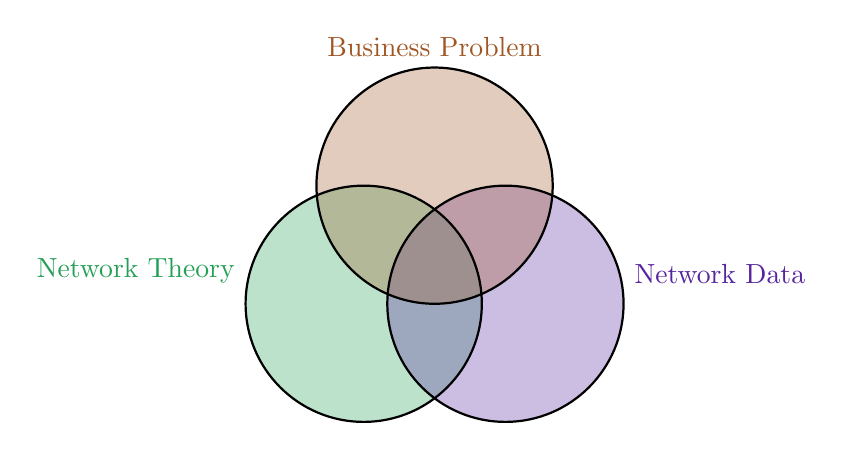
\begin{tikzpicture}[
			thick,
			set/.style = {circle, minimum size = 3cm, opacity=0.3},
			auto,
			->,
			]
			\node[set,label={[text=base_c]175:Network Theory}, fill=base_c] (A) at (0,0) {};
		 	\node[set,label={[text=tri_1]5:Network Data}, fill=tri_1] (B) at (1.8,0) {};
		 	\node[set,label={[text=tri_2]Business Problem}, fill=tri_2] (C) at (0.9,1.5) {};
		  	% circles
		  	\draw (0,0) circle(1.5cm);
	    	 	\draw (1.8,0) circle(1.5cm);
	     	        \draw (0.9,1.5) circle(1.5cm);
		\end{tikzpicture}
	\end{figure}	
\end{frame}

\begin{frame}
\tikzstyle{block} = [
	rectangle, 
	draw,
	text width=8em,
	text centered,
	rounded corners,
	minimum height=2em
	]
\tikzstyle{arrow} = [
	draw,
	-latex',
	rounded corners
	]
\tikzstyle{line} = [
	draw
	]
\tikzstyle{invisible4} = [
	rectangle
	]
\tikzstyle{invisible5} = [
	rectangle
	]
	\frametitle{Where Does a Network Analytics Project Stand?}
	\begin{figure}
		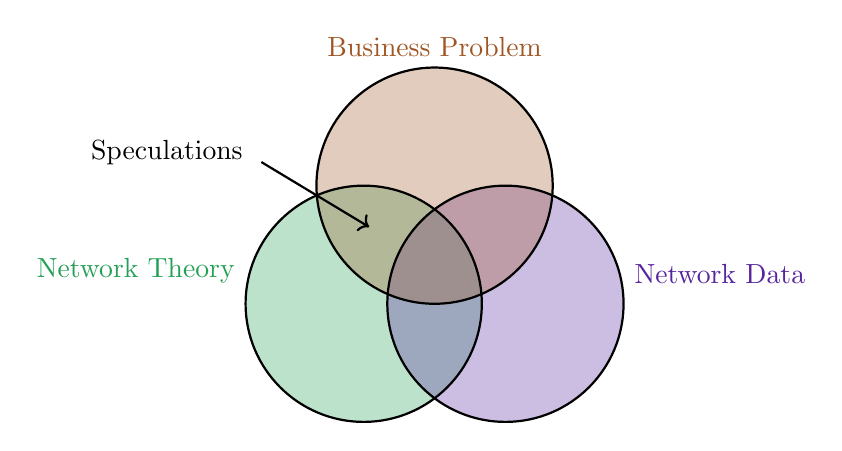
\begin{tikzpicture}[
			thick,
			set/.style = {circle, minimum size = 3cm, opacity=0.3},
			auto,
			->,
			]
			\node[set,label={[text=base_c]175:Network Theory}, fill=base_c] (A) at (0,0) {};
		 	\node[set,label={[text=tri_1]5:Network Data}, fill=tri_1] (B) at (1.8,0) {};
		 	\node[set,label={[text=tri_2]Business Problem}, fill=tri_2] (C) at (0.9,1.5) {};
		  	% circles
		  	\draw (0,0) circle(1.5cm);
	    	 	\draw (1.8,0) circle(1.5cm);
	     	        \draw (0.9,1.5) circle(1.5cm);
			% notes 
			\node[,label={[text=black]Speculations}] (i1) at (-2.5,1.5) {};
			\node[] (p1) at (0.2,.975) {};
			% edges 
			\path[]
			(-1.3,1.8) edge[bend right=0] node [] {} (p1.west)
			;
		\end{tikzpicture}
	\end{figure}	
\end{frame}

\begin{frame}
\tikzstyle{block} = [
	rectangle, 
	draw,
	text width=8em,
	text centered,
	rounded corners,
	minimum height=2em
	]
\tikzstyle{arrow} = [
	draw,
	-latex',
	rounded corners
	]
\tikzstyle{line} = [
	draw
	]
\tikzstyle{invisible4} = [
	rectangle
	]
\tikzstyle{invisible5} = [
	rectangle
	]
	\frametitle{Where Does a Network Analytics Project Stand?}
	\begin{figure}
		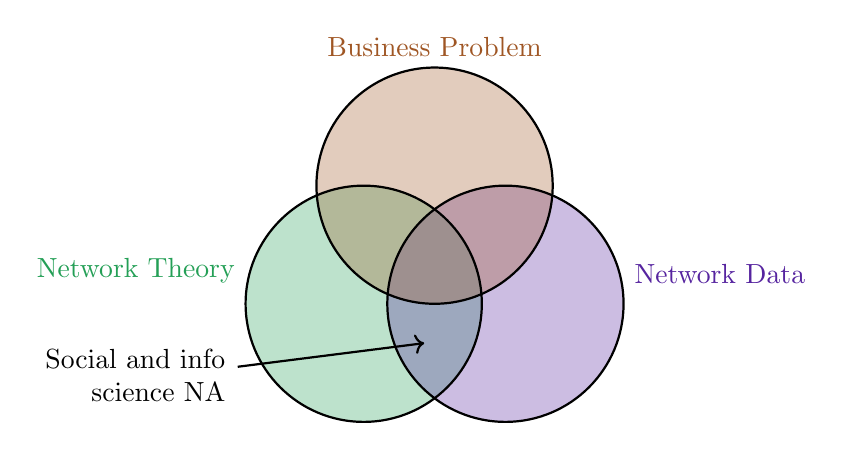
\begin{tikzpicture}[
			thick,
			set/.style = {circle, minimum size = 3cm, opacity=0.3},
			auto,
			->,
			]
			\node[set,label={[text=base_c]175:Network Theory}, fill=base_c] (A) at (0,0) {};
		 	\node[set,label={[text=tri_1]5:Network Data}, fill=tri_1] (B) at (1.8,0) {};
		 	\node[set,label={[text=tri_2]Business Problem}, fill=tri_2] (C) at (0.9,1.5) {};
		  	% circles
		  	\draw (0,0) circle(1.5cm);
	    	 	\draw (1.8,0) circle(1.5cm);
	     	        \draw (0.9,1.5) circle(1.5cm);
			% notes 
			\node[,label={[align=right, text=black]Social and info\\science NA}] 
			      (i4) at (-2.9,-1.5)
			       {};
			\node[] (p4) at (0.9,-0.5) {};
			% edges 
			\path[]
			(-1.6, -0.8) edge[bend right=0] node [] {} (p4.west)
			;
		\end{tikzpicture}
	\end{figure}	
\end{frame}

\begin{frame}
\tikzstyle{block} = [
	rectangle, 
	draw,
	text width=8em,
	text centered,
	rounded corners,
	minimum height=2em
	]
\tikzstyle{arrow} = [
	draw,
	-latex',
	rounded corners
	]
\tikzstyle{line} = [
	draw
	]
\tikzstyle{invisible4} = [
	rectangle
	]
\tikzstyle{invisible5} = [
	rectangle
	]
	\frametitle{Where Does a Network Analytics Project Stand?}
	\begin{figure}
		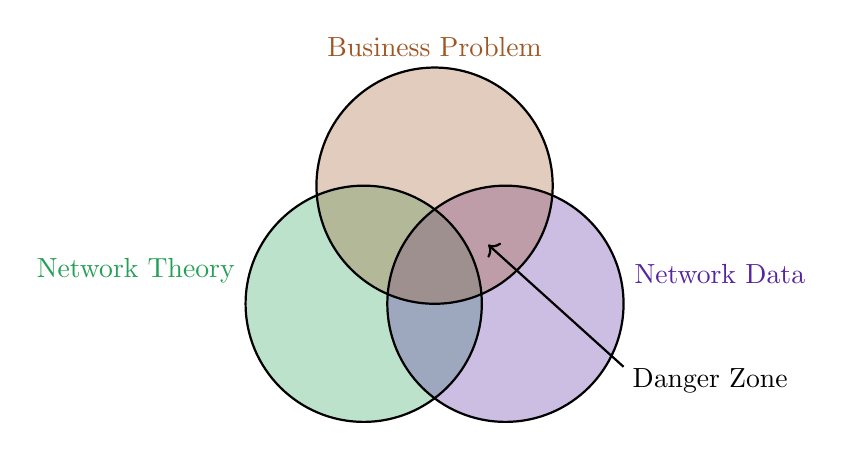
\begin{tikzpicture}[
			thick,
			set/.style = {circle, minimum size = 3cm, opacity=0.3},
			auto,
			->,
			]
			\node[set,label={[text=base_c]175:Network Theory}, fill=base_c] (A) at (0,0) {};
		 	\node[set,label={[text=tri_1]5:Network Data}, fill=tri_1] (B) at (1.8,0) {};
		 	\node[set,label={[text=tri_2]Business Problem}, fill=tri_2] (C) at (0.9,1.5) {};
		  	% circles
		  	\draw (0,0) circle(1.5cm);
	    	 	\draw (1.8,0) circle(1.5cm);
	     	        \draw (0.9,1.5) circle(1.5cm);
			% notes 
			\node[,label={[text=black]Danger Zone}] (i3) at (4.4,-1.4) {};
			\node[] (p3) at (1.45,0.75) {};
			% edges 
			\path[]
			(3.3,-0.8) edge[bend right=0,] node [] {} (p3.east)
			;
		\end{tikzpicture}
	\end{figure}	
\end{frame}

\begin{frame}
\tikzstyle{block} = [
	rectangle, 
	draw,
	text width=8em,
	text centered,
	rounded corners,
	minimum height=2em
	]
\tikzstyle{arrow} = [
	draw,
	-latex',
	rounded corners
	]
\tikzstyle{line} = [
	draw
	]
\tikzstyle{invisible4} = [
	rectangle
	]
\tikzstyle{invisible5} = [
	rectangle
	]
	\frametitle{Where Does a Network Analytics Project Stand?}
	\begin{figure}
		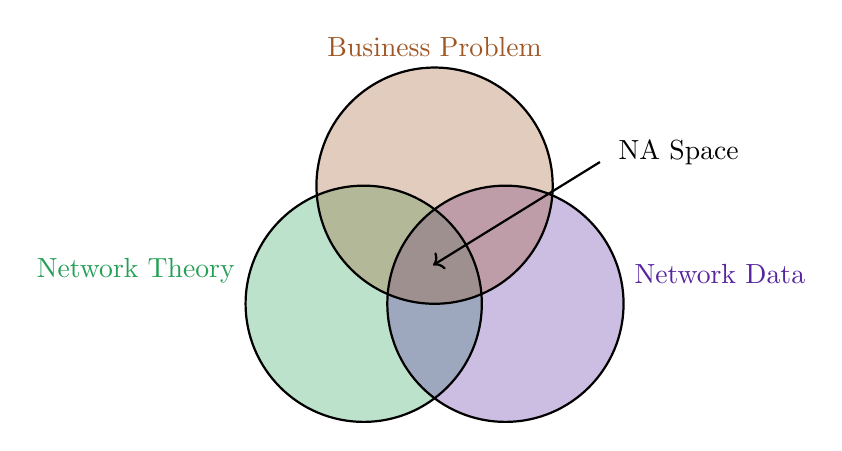
\begin{tikzpicture}[
			thick,
			set/.style = {circle, minimum size = 3cm, opacity=0.3},
			auto,
			->,
			]
			\node[set,label={[text=base_c]175:Network Theory}, fill=base_c] (A) at (0,0) {};
		 	\node[set,label={[text=tri_1]5:Network Data}, fill=tri_1] (B) at (1.8,0) {};
		 	\node[set,label={[text=tri_2]Business Problem}, fill=tri_2] (C) at (0.9,1.5) {};
		  	% circles
		  	\draw (0,0) circle(1.5cm);
	    	 	\draw (1.8,0) circle(1.5cm);
	     	        \draw (0.9,1.5) circle(1.5cm);
			% notes 
			\node[,label={[text=black]NA Space}] (i2) at (4,1.5) {};
			\node[] (p2) at (0.75,0.49) {};
			% edges 
			\path[]
			(3,1.8) edge[bend right=0] node [] {} (p2.east)
			;
		\end{tikzpicture}
	\end{figure}	
\end{frame}

% =========================== The business problem ========================
\section{The Business Problem}

\begin{frame}
	\frametitle{}
	\centering 
	\LARGE What is a business problem?
\end{frame}

\begin{frame}
	\frametitle{Companies Are Not Very Good at Problem Diagnosing}
	\small
	\begin{columns}
		\begin{column}{0.45\textwidth}
			\begin{figure}
				\begin{small}
					\begin{center}
						\includegraphics[
							width=0.95\textwidth
							]{images/problem_diagnosis.png}
					\end{center}
				\end{small}
			\end{figure}
		\end{column}
		\begin{column}{0.45\textwidth}
			There are several concurrent causes:
			\begin{itemize}
				\item 
				The overall tendency to over-engineer the problem 
				diagnosis process constraints the peripheral 
				view of organizations --- thus, 
				unconventional problems could not receive 
				attention!
				\item
				The adoption of time-consuming tools, such as 
				`Six Sigma,' limit the attention and energy 
				organizations can devote to spot 
				problems
				\item 
				Organizations tend tend to dig deeper in problems
				they have already defined 
			\end{itemize}
		\end{column}
	\end{columns}
\end{frame}

\begin{frame}
	\frametitle{Client-Consultancy Interaction is Troublesome}
	\small
	\begin{columns}
		\begin{column}{0.5\textwidth}
			\begin{figure}
				\begin{center}
					\includegraphics[
						width=1\textwidth
						]{images/client_consultancy}
				\end{center}
			\end{figure}
		\end{column}
		\begin{column}{0.5\textwidth}
			The barriers to an effective interaction originate from 
			differences in:
			\begin{itemize}
				\item Frames of reference --- individual organizations 
				develop idyiosyncratic ways of processing information
				\item Goals --- consultancies not necessarily 
				tackle their clients' problems in ways that 
				correspond with their clients' interests
				\item Logics --- consultancies and clients 
				live in different `thought worlds.' For example 
				clients value specialization and industry 
				knowledge much more than consultancies do
			\end{itemize}
		\end{column}
	\end{columns}
\end{frame}

\begin{frame}
	\frametitle{Real World Problem Statements I Worked With}
	\begin{quote}
		``Our data say employees have not come up with 
		fresh ideas for quite a while. We need to find out.''
	\end{quote}
	\raggedleft --- The innovation platform manager of a global public utility.

	\vspace{1em}

	\begin{quote}
		``The people in the [R\&D] department do not part-take in 
		the decision making process regarding the selection 
		of the future projects. Shall they?''
	\end{quote}
	\raggedleft --- The Head of Reserch of a big pharma company.
	\vspace{1em}

	\begin{quote}
		``Engineers want more autonomy in forming a new product 
		development team. What are the pros and cons?''
	\end{quote}
	\raggedleft --- The CTO of a global semiconductor company.
	
\end{frame}

\begin{frame}
	\frametitle{Mapping Business Problems on Objective Functions and Domains}

	\begin{table}
		\begin{small}
			\begin{center}
				\begin{tabular}[c]{
					p{3cm}|p{2.1cm}|p{2.1cm}|p{2.1cm}|p{2.1cm}
					}
					%\hline
					\multicolumn{1}{c}{\textbf{}}
					& \multicolumn{4}{c}{\textbf{Domain}}\\
					\hline
					\textbf{Objective function}
					&\multicolumn{1}{c|}{\textbf{Employee}}
					&\multicolumn{1}{c|}{\textbf{Project}}
					&\multicolumn{1}{c|}{\textbf{Organization}}
					&\multicolumn{1}{c}{\textbf{Inter-orgs}}\\
					\hline
					Creativity\dotfill&
					\cellcolor{white!25}\multicolumn{1}{c}{\bullet}& 
					\cellcolor{white!25}\multicolumn{1}{c}{\bullet}&
					&
					\\ 
					% \cline{2-5}
					Knowledge sharing\dotfill&
					\cellcolor{white!25}\multicolumn{1}{c}{\bullet}&
					\cellcolor{white!25}\multicolumn{1}{c}{\bullet}&
					&
					\\
					% \cline{2-5}
					Task performance\dotfill&
					\cellcolor{white!25}\multicolumn{1}{c}{\bullet}&
					\cellcolor{white!25}\multicolumn{1}{c}{\bullet}&
					&
					\\ 
					Coordination\dotfill&
					\cellcolor{white!25}\multicolumn{1}{c}{\bullet}&
					\cellcolor{white!25}\multicolumn{1}{c}{\bullet}&
					\cellcolor{white!25}\multicolumn{1}{c}{\bullet}&
					\cellcolor{white!25}\multicolumn{1}{c}{\bullet}\\
					% \cline{2-5}
					Innovation\dotfill&
					\cellcolor{white!25}\multicolumn{1}{c}{\bullet}&
					\cellcolor{white!25}\multicolumn{1}{c}{\bullet}&
					\cellcolor{white!25}\multicolumn{1}{c}{\bullet}&
					\cellcolor{white!25}\multicolumn{1}{c}{\bullet}\\ 
					% \cline{2-5}
				        Econ performance\dotfill&
					&
					&\cellcolor{white!25}\multicolumn{1}{c}{\bullet}
					&
					\\
					% \hline
				\end{tabular}
			\end{center}
		\end{small}
	\end{table}
	\textit{Notes.} --- The table shows common associations between business problems' 
	objective functions (what clients want to achieve in essence) 
	and domains (the level at which the problem should be addressed). Dots 
	denote the existence of common associations.
\end{frame}

% =========================== Network theory ==============================
\section{Network Theory}

\begin{frame}
	\frametitle{The Goals of Network Theory}
	Mainly, network theory aims to explain

	\begin{enumerate}
		\item Why some nodes or groups achieve more (the 
		social capital tradition)
		\item Why some nodes or  networks  are  more  similar  to  
		each  other  (the  social   homogeneity   tradition)
	\end{enumerate}
	
\end{frame}

\begin{frame}
	\frametitle{Network Theory's Network Views}

	Network theories mirror two different views of networks

	\begin{itemize}
		\item The first view --- known as the `network flow model' 
		--- emphasizes the information, resources, or artefacts 
		that flow through the network and possibly accrue to 
		the individual nodes
		\begin{itemize}
			\item \textit{Sample proposition}: central nodes have an information advantage
			over peripheral ones
		\end{itemize}
		\item The second view --- known as the `network architecture 
		model' --- highlights the connection between network structure 
		and individual or organizational outcomes  
		\begin{itemize}
			\item \textit{Sample proposition}: decentralized organizational 
			structures are more suited in high-tech industries than
			low-tech companies
		\end{itemize}
	\end{itemize}
\end{frame}

\begin{frame}
	\frametitle{Groups of Network Theories}
	\centering
	\small
	\begin{table}
		\begin{center}
			\begin{tabular}[c]{l|l|l}
				% \hline
				\textbf{Underlying model} & 
				\textbf{Social capital} &
				\textbf{Social homogeneity}\\
				\hline
				\textbf{Network flow} & Capitalization (value creation) & Contagion  \\
				\hline
				\textbf{Network architecture} & Coordination & Adaptation  (network change)\\
				% \hline
			\end{tabular}
		\end{center}
	\end{table}

	\vspace{1em}

	\raggedright \small Source is~\cite[][page 47]{scott2011}
\end{frame}

\begin{frame}
	\frametitle{Network Theories across the Various Weeks of SMM638}
	\begin{table}
		\begin{tabular}[c]{l|c|c|c|c|c|c|c|c}
			% \hline
			\textbf{Network theory} & 
			\textbf{2} & 
			\textbf{3} & 
			\textbf{4} & 
			\textbf{5} & 
			\textbf{7} & 
			\textbf{8} & 
			\textbf{9} & 
			\textbf{10}\\
			\hline
			Value creation &  & \bullet & &  &  &  &  & \\	
			Coordination &  &  &\bullet  & \bullet &  &  &  & \\	
			Network change &  &  &  &  & \bullet & \bullet & \bullet & \bullet\\	
			Contagion &  &  &  &  &  & &  & \bullet \\	
			% \hline
		\end{tabular}
	\end{table}
\end{frame}

% =========================== Network data ================================
\section{Network Data}

\begin{frame}
	\frametitle{Representing Network Data: Some Caveats}
	\begin{itemize}
		\item 
		All across the various weeks of the module, we will spend substantial time to
		represent various relations in network terms 
		\item 
		Such a representation exercise is all but trivial --- oftentimes, we have to carefully
		consider the characteristics of the relation at the center of a network
		\item 
		In order to facilitate the `network representation exercise,' it is particularly useful
		to reason with some stylized networks
		\item 
		Particularly, there are some differentiating dimensions, say features, that we may want to consider 
		in order to understand `what form of network we are dealing with'
	\end{itemize}
\end{frame}

\begin{frame}
	\frametitle{Forms of Networks}
	It is socially accepted to distinguish networks between

	\begin{itemize}
		\item 
   		Directed Vs undirected
		\item
   		Weighted Vs unweighted
		\item  		
		One Vs two-mode
	\end{itemize}
	
	\vspace{1em}

	\begin{tcolorbox}[
		colback=comp_c!5!white,
		colframe=comp_c!90!black,
		title={\centering !! Pay attention !!}]
		These categories are not mutually exclusive. E.g., a network can be 
		both directed and weighted.
	\end{tcolorbox}
	
\end{frame}


\begin{frame}
	\frametitle{Directed Vs Undirected Networks}

	Key features

		\begin{itemize}
			\item A network is directed when there is a sender and a 
			receiver node, undirected otherwise
			\item Soundcloud's following network is an example of a
			directed network 
			\item `Friendship' is tipically represented as an undirected
			network
		\end{itemize}

\end{frame}

\begin{frame}
	\frametitle{Weighted Vs Unweighted Networks}

	Key features

		\begin{itemize}
			\item A network is weighted when edges have a numerical value
			(i.e., not all edges are born equal)
			\item Information sharing is an example of a
			weighted network 
			\item `Friendship' is tipically represented as an unweighted
			network
		\end{itemize}

\end{frame}

\begin{frame}
	\frametitle{One- Vs Two-Mode Networks}

	Key features

		\begin{itemize}
			\item A network is one-mode when it contains the nodes 
			of the same type, two-mode otherwise
			\item Soundcloud's following network is an example of a
			one-mode network 
			\item Soundcloud's like network is an example of a two-mode
			network
		\end{itemize}

\end{frame}

\begin{frame}
	\frametitle{Algebric Representations for Network Data}

	The adjacency matrix for a one-mode, directed, unweighted network

        \begin{equation}
        A_{i,j} = 
         \begin{pmatrix}
          0 & 1 & 0 & 0 & 0 \\
          0 & 0 & 0 & 0 & 1 \\
          0 & 0 & 0 & 1 & 0 \\
          0 & 0 & 0 & 0 & 1 \\
          0 & 0 & 0 & 0 & 0 \\
         \end{pmatrix}
        \end{equation}
	
\end{frame}

% =========================== Session 2 wrapup =============================
\section{Session 2 Wrap Up}

\begin{frame}
	\frametitle{}
	\LARGE \center What have we learned today?
\end{frame}

% =========================== Bibliography =================================

\begin{frame}
	\frametitle{References}
	\printbibliography
 \end{frame} 

\end{document}